\documentclass[a4paper,11pt,uplatex]{jsbook}

\newcommand{\V}[1]{\boldsymbol{#1}}
\def\thline{\noalign{\hrule height 1pt}}
\def\tvline{\vrule width 1pt}

\usepackage{makeidx}
\usepackage{amsmath}
\usepackage{amssymb}
\usepackage[dvipdfmx]{graphicx}
\usepackage{float}
\usepackage{bm}

\makeindex

\pagenumbering{roman}

\begin{document}
\title{平成27年度 修士論文\\
 \\
移動ロボットのための\\
不確かさを考慮した障害物回避行動の生成}
\author{鈴木勇矢\\
Chiba Institute of Technology}
\date{2020年2月x日}

% \maketitle
% \chapter*{謝辞}\addcontentsline{toc}{chapter}{謝辞}

和文だとうしろに持っていくことが多いのですが、
私は前のほうが好きです。


南武線に感謝します。

横須賀線に感謝します。

総武線に感謝します。

京葉線に吹き付ける横風に感謝します。


% \tableofcontents

%%% 本文 %%%
% 章のページの先頭は左側(奇数ページ)に来る
% \cleardoublepage
\pagenumbering{arabic}

% \chapter{序論} \label{chapter:introduction}


%%%%%%%%%%%%%%%%%%%%%%%%%%%%%%%%%%%%%%%%%%%%%%%%%%%%%%%%%%%%%%%%%%%%%%%%%%%%%%%%
\section{背景} \label{section:backglound}

\index{うえだ@上田} %消すとコンパイルできない
人間による操縦を必要とせず, 自律的に活動するロボットに対する社会の期待が高まっている. 
自律ロボットの活躍が期待される場所は多岐に渡り, 従来のロボットのように工場のラインだけでなく, 住宅や商業施設, あるいは被災地のような極限環境も含まれる. 
ロボットには様々な種類が存在するが, 中でも自律移動ロボットは, 病院内の搬送や空港の警備などの用途で, すでに社会実装されたものも多く存在する. 

これらの環境で移動ロボットが自律的に活動するためには, 自己位置や周辺環境の把握と行動計画を行う必要がある. 
実世界で活動するロボットは, 自身の位置を直接知ることはできない.  %あとで
したがって, 搭載したセンサを用いて自身の位置や周辺環境を把握する必要がある. 
そして, ロボットは把握した自己位置や環境の情報を頼りに, 目標地点へと移動するための行動を計画し動作する. 

しかしながら, 移動ロボットの活躍が求められている環境の多くは複雑で, 不確かな要素が多く存在する. 
人間の生活する空間は, 工業の組み立てラインのように不確かさや誤差がなるべく小さくなるように精密に構成されてはいない. 
また, センサが知覚できる情報には限りがありノイズが含まれているため, ロボットが環境の情報を完全に知覚することはできない. 
アクチュエータにおいても, 制御ノイズや消耗のような要因から誤差が存在し, モデル化やアルゴリズムの近似による誤差も存在する. 
したがって, ロボットが実世界で自律的に活動するためには, これら多くの不確かさに対処していく必要がある. 

不確かさを考慮するためには, 確率論に基づく方法が有効である. 
ロボティクスにおいて, 確率論を用いて不確かさに対処する試みは「確率ロボティクス(Probabilistic Robotics)」と呼ばれ, 盛んに研究が行われている\cite{thrun2005,上田2007prob}. 
確率ロボティクスは, ロボットの知覚と制御に確率・統計を駆使することで, ロボット技術において避けて通ることができない不確かさを陽に表現することを可能としている. 
移動ロボットにおいて重要な自己位置推定や行動計画についても, 不確かさを考慮した様々なアルゴリズムが提案されている. 

この確率論に基づく自己位置推定には, ベイズフィルタが有効であると示されている. 
確率ロボティクスでは, ロボットの自己位置を決定論的な一つの位置ではなく, 空間中における確率分布として表現する. 
ベイズフィルタによる自己位置推定では, ベイズの定理に基づき, 確率分布を逐次更新していく. 
この分布は信念分布と呼ばれ, ロボットが得られる情報をもとに, 主観的に自身の位置をどのように信じているかを表している. 

現在, 多くの移動ロボットにおいて, 確率論に基づく自己位置推定が取り入れられている. 
中でもとくに, Monte Carlo localization (MCL) という手法が多く利用されている\cite{dellaert1999, fox1999}. 
これは, ベイズフィルタによるロボットの自己位置推定を実装する方法の1つである. 
MCLでは, ロボットの信念分布を位置と姿勢からなる空間中に分布させた重みを持つ粒子(パーティクル)で近似的に表現する. 
これにより, ロボットの信念を複雑な確率分布として表現することを可能としている. 
同じくベイズフィルタを理論的背景としたカルマンフィルタによる自己位置推定では, 信念は正規分布でしか表現できない\cite{kalman1960}. 
対して, MCLでは一様や多峰性の分布などを表現することが可能であるため, 複雑な環境で活動することが求められる移動ロボットに適している. 
ロボット開発用のミドルウェアであるROSでは, LiDARと専有格子地図を用いたMCLによる自己位置推定のプログラムが, 標準のナビゲーションパッケージとして用意されており, 多くの開発者や研究者に利用されている\cite{quigley2009ros,roswiki_amcl}. 
また, 実環境において移動ロボットに自律移動を行わせる技術チャレンジであるつくばチャレンジでは, 多くのチームがLiDARと専有格子地図用いたMCLを用いている. 
\cite{夏迫2016つくばチャレンジ}
これらのことからも, MCLは実環境における自律移動ロボットの自己位置推定の手法として, 有効であることが分かる. 

現在, 様々な自律移動ロボットにおいて確率的な自己位置推定手法が取り入れられている一方で, 行動決定においては不確かさについて考慮されないことがある. 
一般的に多くの自律移動ロボットは, MCLやカルマンフィルタにより自身の位置を確率分布として推定する. 
そして, 最も確率の高い位置を自身が存在する真の位置だと仮定し, 行動計画を行う. 
しかし, このような方法では, ロボットの自己位置推定により得られた確率的な情報が, 行動決定に反映されない. 
ロボットは信念分布が大きい場合も, 分布が推定誤差が小さい場合も, 同様の行動を行うことになる. 
% たとえば, つくばチャレンジにおいて, 曲がり角で内側の段差にタイヤがははまり込みリタイアとなった例がある. (以前話で聞いただけなので参考となる文献を探す)

ロボット同様に, 実世界で活動する我々にとっても不確かさは避けることができない問題だが, 
人間や一部の動物は, 得られる情報が制限されている状況下でも, 適切な行動を選択する. 
たとえば, 人間は壁沿いを移動することで暗闇の中でも寝室に向かうことが可能であり, 
明るく視界に制限がないときとは異なる動作を行うことで, 不確かさに対処している. 
このように状況に合わせた自律的な行動をロボットに行わせるためには, 行動決定アルゴリズムで不確かさを考慮することが必要である. 


%%%%%%%%%%%%%%%%%%%%%%%%%%%%%%%%%%%%%%%%%%%%%%%%%%%%%%%%%%%%%%%%%%%%%%%%%%%%%%%%
\section{先行研究} \label{section:related works}

不確かさに応じた柔軟な行動決定をロボットに行わせることができると, 得られる情報が制限された状況下でもタスクを実行させることが可能となる. 
ロボット工学では, 部分観測マルコフ決定過程(POMDP)という枠組みで研究されているが, 計算量の観点から最適な解を導くことができないと知られている\cite{kaelbling1998}. 
そこで, 近似的にPOMDPを解く手法が複数提案されている. 

暗闇の中, 壁伝いに寝室へ向かうような行動については, Royらによって提案された手法によりロボットへと実装されている\cite{roy1999b}. 
この手法では, ロボットは事前に4次元の状態空間において行動計画が行われる. 
状態は, X-Y平面上ロボットの位置と方向に, 推定の不確かさの大きさを表すスカラー値を足した, 4つで表される. 
計画された行動には, 推定の不確かさを小さく保ちながらゴールへと向かう特性が現れた. 
この研究では, ロボットの自己位置推定は壁との距離を測定することで行われるため, ロボットは壁から大きく離れないようにゴールへと向かう動作を行った. 
この手法は, 沿岸航法(coastal navigation)と呼ばれる. 

Littmanらによって提案された$Q_{\rm MDP}$ value method\cite{littman1995}は, 事前の行動計画と観測の不確かさを分けて扱った. 
Q-MDP法では, 観測の不確かさを考慮せずに, マルコフ決定過程の問題としてロボットの行動を事前に計画し, 
実際にロボットが行動を決定するときに, 観測の不確かさを考慮する. 
事前に計画した行動と現在の信念の確率分布から, 各行動に対する期待値計算を行い, 最も良い行動を選択する. 

$Q_{\rm MDP}$ value methodは, Uedaらによって実際のロボットへと実装された\cite{ueda2003iros}. 
RoboCupの四足歩行リーグのゴールキーパーのロボットへと適用され, 有効性が示された. 

Uedaによって提案されたPFC法では, 移動ロボットがゴールを探索するような動作を可能にしている\cite{ueda2015}. 
この手法では, $Q_{\rm MDP}$ value methodの行動評価の式に変更を加えることで, ゴールに近いパーティクルが行動決定に及ぼす影響を大きくする. 
これにより, ロボットは自身の位置がほぼ分からない状況から, パーティクルにより近似された信念を徐々にゴールに流し込むような動作を行う. 
分布が徐々にゴールに吸い込まれるように移動していき, ロボットが分布の中にいる場合, ロボットもその流れに従いゴールへと到達する. 
また, ゴール付近のパーティクルが行動決定に及ぼす影響の大きさを変更した際に, 
$Q_{\rm MDP}$ value methodで問題となっていた, ローカルミニマムによる行動の停滞が起こる頻度が低下することについても示されている\cite{ueda2018searching}. 

PFC法は, 障害物が存在しない空間において, 自己位置推定が極めて不確かな移動ロボットのナビゲーションに有効であることが, シミュレーション実験において示されている. 
しかし, 障害物が存在する環境での動作については, 有効性は確認されていない. 
PFC法では, ゴール付近のパーティクルが行動決定に及ぼす影響を大きくする一方で, 
ゴールから遠いパーティクルや障害物内に存在するパーティクルは, 軽視されることになる. 
つまり, ロボットが障害物を回避しようとする行動は反映されにくいという性質がある. 
一般的に, 自律移動ロボットが活動することが求められている環境には, 動的なものや静的なものを含め, 多くの障害物が存在する. 
移動ロボットのナビゲーションでは, 障害物の回避について考えることが必要であると言える. 


\section{目的}
そこで本研究では, 自己位置推定の不確かさを考慮した障害物の回避行動を自律移動ロボットに行わせるための手法を提案する. 
PFC法に変更を加えることで, 信念を近似するパーティクル全体が障害物を回避するような動作を生成する. 
これにより, 自律移動ロボットに自己位置推定の不確かさを考慮した障害物回避の行動をとらせつつ, ゴールを探索するような動作を行わせることを可能にする. 
また, その有効性について通常のPFC法と比較することで検証する. 


%%%%%%%%%%%%%%%%%%%%%%%%%%%%%%%%%%%%%%%%%%%%%%%%%%%%%%%%%%%%%%%%%%%%%%%%%%%%%%%%
\section{本論文の構成}
まず, 第\ref{chapter:introduction}章では, 本研究の背景と先行研究を述べ, 目的を設定した. 
第\ref{chapter:localization}章では, ロボットの状態推定について述べる. 
第\ref{chapter:pomdp}章では, 不確かさを考慮したロボットの行動決定について述べ, 
第\ref{chapter:method}章では, 提案する手法について述べ, 
第\ref{chapter:evaluate}章では, 提案手法をPFC方と比較し評価する. 
最後に第\ref{chapter:conclusion}章で, 本論文のまとめを述べる. 


% \begin{figure}[ht]
%   \begin{center}
%     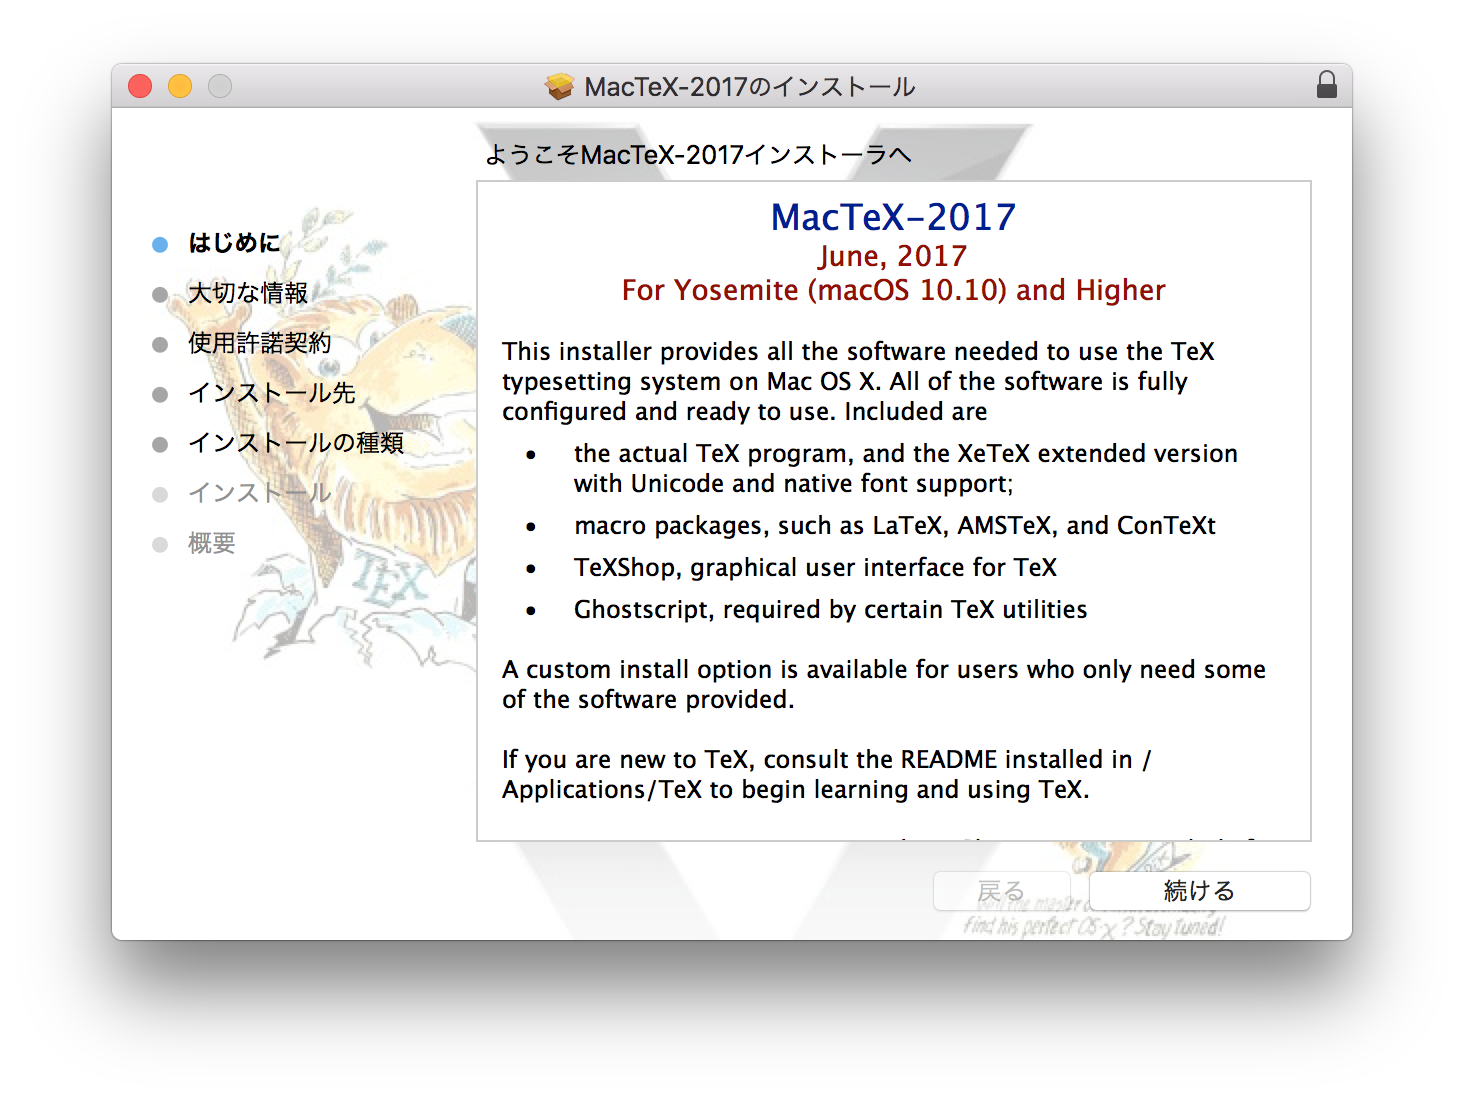
\includegraphics[width=10cm, ]{figs/image.png}
%   \end{center}
% \end{figure}

% \chapter{MCLによる移動ロボットの自己位置推定} \label{chapter:localization}

本章では, ベイズフィルタによる移動ロボットの自己位置推定手法の一つである, Monte Carlo localization (以下MCL)について述べる. 
MCLの概要について述べ, 各処理の処理内容を説明する. 
本論文において, 移動ロボットの自己位置推定にはMCLが利用されるものとする. 


%%%%%%%%%%%%%%%%%%%%%%%%%%%%%%%%%%%%%%%%%%%%%%%%%%%%%%%%%%%%%%%%%%%%%%%%%%%%%%%%
\section{MCLの概要}

MCLは, ベイズフィルタを理論的背景としたロボットの自己位置推定手法の1つである. 
MCLでは, 表現したい任意の空間上$\mathcal{X}$上に存在する確率密度関数を, 空間上に散布した標本により表現することで, ロボットの姿勢を確率的に推定する. 
この標本はパーティクル(粒子)と呼ばれ, ロボットの信念分布を表す確率密度関数$b_t(\bm{x})$を近似するように配置される. 
各パーティクルは変数としてロボットと同次元の姿勢$\bm{x}$と重み$w$の情報を持っており, $N$個のパーティクルの集合は
\begin{equation}
\label{particles}
  % \Xi_{t} = \{ \xi^{(i)}_{t} = (\bm{x}^{(i)}_{t}, w^{(i)}_{t}) |i = 1,2,\dots,N \}
  \Xi = \{ \xi^{(i)} = (\bm{x}^{(i)}, w^{(i)}) |i = 1,2,\dots,N \}
\end{equation}
のように定義される. 
基本的に全パーティクルの重みの合計は, 常に
\begin{equation}
\label{weight_sum}
  \sum_{i=1}^{N}w^{(i)}_{t}=1
\end{equation}
を保つように実装される. 

ロボットの状態を表す変数については様々存在するが, 自己位置推定ではロボットの姿勢(位置と向き)を推定する. 
本論文では, 二次元平面を低速で移動する対向二輪型の移動ロボットを想定し, ロボットの二次元平面上における位置$(x, y)$と向き$\theta$をあわせた3次元の状態$\bm{x} = (x, y, \theta)$の推定について扱う. 
したがって, ロボットの姿勢と同様に, パーティクルの姿勢はそれぞれ$\bm{x}^{(i)} = (x^{(i)}, y^{(i)}, \theta^{(i)})$となる. 

MCLのアルゴリズムは, 主に次の4ステップからなる. 
2から4を繰り返し行うことで逐次ロボットの姿勢を推定する. 
\begin{enumerate}
  \item 初期化
  \item 動作による更新
  \item 計測による更新
  \item リサンプリング
\end{enumerate}


%%%%%%%%%%%%%%%%%%%%%%%%%%%%%%%%%%%%%%%%
\section{初期化}

初期化のステップでは, パーティクルの初期化を行う. 
N個のパーティクルの初期姿勢$\bm{x}^{(i)}$を決定し, 重み$w^{(i)}$を$1/N$とする. 
パーティクルのばらまき方は, ロボットの初期の信念分布に従うように行う. 
一般的には, 以下のようなパーティクル初期姿勢の決定方法が用いられる. 

ロボットを人間が自由に配置する場合など, 初期姿勢が予め分かっている場合は, ロボットの信念分布をロボットが存在すると考えられる位置を平均とした正規分布と考え, 
パーティクルの初期姿勢$\bm{x}^{(i)}$を平均$\mu$, 分散$\Sigma$の正規分布に従うように決定する. 
本論文における移動ロボットの自己位置推定では, 状態$\bm{x}^{(i)}$が位置と向きからなる3次元のため, $\bm{\mu}$と$\Sigma$はそれぞれ3次元ベクトル, $3\times3$の分散共分散行列として扱う. 
多くの場合$\bm{\mu}$と$\Sigma$はヒューリスティックに決定する. 

一方, ロボットの初期位置が完全に不明なとき, ロボットの初期信念分布は状態空間$\mathcal{X}$全体の一様分布と考えられる. 
その場合は, パーティクルの姿勢は一様分布に従うように配置する. 

% MCLは, ロボットの制御出力や移動量, センサに含まれるノイズに頑健な推定が行える. 
% しかし, 想定を上回るノイズが混入した場合に, ロボットの真の姿勢$\bm{x}^{(*)}$とパーティクルの分布$\Xi$が大きく乖離することがある. 
% MCLでは, パーティクルの分布がロボットの真の位置$\bm{x}^{*}$がから大きく離れることがある. 
% このようなロボットの真の姿勢の周辺にパーティクルが存在しない状態は, 「誘拐状態」と呼ばれる. 
% 誘拐状態となったとき, 一般的にはふたたびパーティクルが真の姿勢周辺に戻ることは少ないとされ, 推定が大きく誤った状態が続く. 
% そこで, 融解状態から回復するための研究が複数行われている. 
% 本論文では, ロボット


%%%%%%%%%%%%%%%%%%%%%%%%%%%%%%%%%%%%%%%%
\section{動作による更新}

動作による更新のステップでは, ベイズフィルタにおける予測ステップを, 各パーティクルに対して行う. 
移動ロボットの状態遷移にはノイズが伴うため, 同様の制御入力でも試行ごとに異なる状態遷移結果となる. 
したがって, ロボットが動作すると信念分布が広がることになる. 
この広がった信念分布を表現するように, パーティクルの分布を更新する. 
各パーティクルの状態をロボットの動作モデル
ロボットの状態遷移確率$p(\bm{x} | \bm{x}_{t-1}, \bm{u}_{t})$とすると, 
動作後の各パーティクルの姿勢は
\begin{equation}
\label{particle trans prob}
  \bm{x}^{(i)}_{t} \sim p(\bm{x} | \bm{x}_{t-1}, \bm{u}_{t})
\end{equation}
のように更新される. 


%%%%%%%%%%%%%%%%%%%%%%%%%%%%%%%%%%%%%%%%
\section{計測による更新}

計測による更新のステップでは, ベイズフィルタにおける計測更新ステップを行う. 
センサにより得られた情報が, 各パーティクルの状態で得られる確率を計算し, 重み$w^{(i)}$を更新する. 
重みの更新はベイズの定理を用いて
\begin{equation}
\label{weight}
  w^{(i)}_{t} = q(\bm{z}_{t} | \bm{x}^{(i)}_{t}) \hat{w}^{(i)}_{t}
\end{equation}
のように計算される. 
尤度関数$q(z_{t} | \bm{x}^{(i)}_{t})$は, 使用するセンサの観測モデルをもとに決定する. 

現在, 移動ロボットの自己位置推定のために, LiDARと呼ばれる光センサによる測距センサや, RGB-Dカメラが広く利用されている. 
これらのセンサを自己位置推定位に用いるロボットは, 条件が揃えば非常に正確な推定を行うことが可能である. 
しかし, 本論文では移動ロボットの状態推定が不確かなときに有効となるような行動決定の手法を提案することを目的としている. 
したがって, 移動ロボットが曖昧にしか状態推定を行えない状況を想定するために, ロボットはこれらのセンサを搭載していないものとする. 

代わりに, ロボットはタスクの終了を検知することができるものとする. 
この仮定は, \ref{chapter:method}章で述べる提案手法, およびその先行研究となるPFC法で必要となる. 
ロボットは, 自身がゴールに到達したか否かを各ステップごとに知ることができ, その情報を計測による更新に用いることができるものとする. 

%%%%%%%%%%%%%%%%%%%%%%%%%%%%%%%%%%%%%%%%
\section{リサンプリング}
リサンプリングステップでは, パーティクルを再配置し重みを均一にする. 
再配置するパーティクルは, 重みに従った確率で選択される. 
重みの小さいパーティクルを間引き, 重みの大きいパーティクルの位置に多くのパーティクルを配置する. 
この操作により, 一箇所に重みが偏り続け推定の精度が下がることを防ぐ. 

パーティクルの選択(サンプリング)にはいくつかの手法が存在する. 
本論文では, 系統抽出法によるリサンプリングを用いる. 

% \chapter{不確かさを考慮した行動決定} \label{chapter:pomdp}

本章では, 不確かさを考慮した行動決定について述べる. 
\ref{section:ロボットの行動決定}節では, ロボットの行動決定について述べる. 
\ref{section:mdp}節では, 状態が既知のロボットの行動決定を扱う枠組みである「マルコフ決定過程について述べる. 
\ref{section:pomdp}節では, ロボットの状態が不確かにしか分からない状況での行動について扱う枠組みである
「部分観測マルコフ決定過程」について述べる. 
\ref{section:q-mdp}節と\ref{section:PFC法}節では, 
本研究の先行研究となる, $Q_{\rm MDP}$ value methodおよびPFC法について述べる. 

% 本章では, 不確かさを考慮した行動決定について述べる. 
% まず, 状態が既知のロボットの最適な行動決定を扱う枠組みである「マルコフ決定過程」について述べる. 
% その後, ロボットの状態が不確かにしか分からない状況での最適な行動を扱う枠組みである「部分観測マルコフ決定過程」について述べる. 
% 最後に, 「部分観測マルコフ決定過程」を近似的に解く手法について, いくつかあるうち, 本研究と関連のあるQ-MDP法およびPFC法について述べる. 


%%%%%%%%%%%%%%%%%%%%%%%%%%%%%%%%%%%%%%%%%%%%%%%%%%%%%%%%%%%%%%%%%%%%%%%%%%%%%%%%
\section{ロボットの行動決定} \label{section:ロボットの行動決定}
本節では, ロボットの行動決定について考える. 
本論文で扱うような移動ロボットの行動決定は, 現在のロボットの位置から目的地までの最短経路を算出して移動する, 「経路計画問題」として扱われる. 
ダイクストラ法やA*法, 人工ポテンシャル法といった多くの手法が提案されており, 現在でも研究が行われている. 
一般的にロボットの経路計画問題では, ロボットの観測や移動は決定論的なもとのして扱われ, 経路が算出される. 

しかし, これまで述べたとおり, 移動ロボットは多くの不確かさを有している. 
移動ロボットに最短の経路を算出して移動するだけでなく, これらの不確かさを考慮した上でさらに知的な動作を行わせる方法について考える必要がある. 
たとえば, 人間であれば, 最短ではあるが危険でゴールに到達できる可能性が低い道よりも, 多少遠回りではあるが高確率で安全にゴールできる道を選択するような, 
「急がば回れ」が有効な場合も存在する. 
あるいは, 自身の位置が正しく把握できていない場合に, 安全を優先し全く動かないでいるよりも, 
多少の危険を冒しとりあえず行動してみてタスク達成を目指す方が有効であるような場合も考えられる. 

このような知的な行動を, 単純に経路計画問題として考えることは困難である. 
そこで本章では, ロボットの移動と経路計画について, 
より一般化した枠組みである(有限)マルコフ決定過程および部分観測マルコフ決定過程について述べる. 

%%%%%%%%%%%%%%
%%%%ロボットの不確かさは大きく分けて, 動作に関するものと観測に関するものの2つに分類できる. 


%%%%%%%%%%%%%%%%%%%%%%%%%%%%%%%%%%%%%%%%%%%%%%%%%%%%%%%%%%%%%%%%%%%%%%%%%%%%%%%%
\section{マルコフ決定過程} \label{section:mdp}
本節では, 移動ロボットの現在の自己位置$\bm{x} \in \mathcal{X}$が既知という前提での行動決定についての定式化を行う. 
このような問題は, マルコフ決定過程(Markov decision process, MDP)という枠組みで議論される. 
時間やロボットの状態等を連続系ではなく離散系で考える場合は, 有限マルコフ決定過程と呼ばれる. 

%%%%%%%%%%%%%%%%%%%%%%%%%%%%%%%%%%%%%%%%
\subsection{状態と終端状態}
\ref{chapter:localization}章で述べたものと同様に, 
状態変数$x,y,\theta$からなる状態空間$\mathcal{X}$を定義する. 
ロボットは自身の現在の状態ベクトル$\bm{x} \in \mathcal{X}$が分かっているものとし, 観測の不確かさについては考慮しない. 

ロボットのタスクには必ず終わりがあるとし, 
ロボットの状態が, 事前に定めたある状態になったときをタスクの終了とする. 
このタスクが終了する状態は, 終端状態と呼ばれ, 終端状態の集合は$\mathcal{X}_f \subset \mathcal{X}$と表現される. 
終端状態は, 移動ロボットの経路計画問題における, ゴールや目標地点などのロボットが目指すべき望ましい状態だけでなく, 陥りたくない状態も含まれる. 

%%%%%%%%%%%%%%%%%%%%%%%%%%%%%%%%%%%%%%%%
\subsection{行動と状態遷移}
ロボットは有限子の制御指令の中から, 一つを選択することで動作する. 
MDPではこの制御指令のことを行動と呼ぶ. 
ロボットの行動は$m$種類存在し, 行動の集合は, 
\begin{equation}
\label{action}
  \mathcal{A} = \{ a_{1}, a_{2}, \ldots , a_{m} \}
\end{equation}
と表現される. 

時間は離散的に表現され, タスクの開始からは終わりまでは${0,1,2,\ldots,t_{f}} \equiv T$と定義される. 
ロボットが最初に行動を選択する時刻を$t=0$とし, 行動が実行されるたびに$t=1,2,\ldots$と次のステップへと進んでいく. 
ロボットが終端状態に入りタスクが終了する時刻を$t_{f}$とする. 
$t_{f}$は固定ではなく, タスク達成までにかかった時間により異なる. 
また, 「時刻$t-1$の状態」, 「時刻$t$に遷移するために選択された行動」, 「時刻$t$の状態」をそれぞれ$\bm{x}_{t-1}, a_{t}, \bm{x}_{t}$と表現する. 
しかし, MDPで扱うシステムは時不変であるため, 多くの場合$t$の具体的な値は重要でははない. 
したがて, 今後はこれらをそれぞれ$\bm{x}, a, \bm{x}^{\prime}$と表記する. 

ロボットの状態$\bm{x}$は, ある行動$a$により状態$\bm{x}^{\prime}$へと遷移する. 
状態の遷移にはノイズが含まれているものとし, 状態と行動が同一の$(\bm{x}, a)$であっても, 事後状態$\bm{x}^{\prime}$は各試行ごとに異なる. 
ロボットの状態遷移は, マルコフ性を持ち, 
\begin{equation}
\label{trans prob}
  \bm{x} \sim p(\bm{x} | \bm{x}_{t-1}, \bm{u}_t) (t=1,2,\ldots,t_{f})
\end{equation}
に従うものとする. 
また, ロボットが$\bm{x}$から行動$a$により$\bm{x}^{\prime}$に遷移する確率を$p^{a}_{\bm{x}\bm{x}^{\prime}}$と表現する. 
この確率$p^{a}_{\bm{x}\bm{x}^{\prime}}$が, $\bm{x}, a, \bm{x}^{\prime}$のあらゆる組に対して既知であり, 時不変であると仮定する. 

%%%%%%%%%%%%%%%%%%%%%%%%%%%%%%%%%%%%%%%%
\subsection{報酬} \label{subsection:reward}
状態$\bm{x}$で行動$a$を行った場合に, 状態が$\bm{x}^{\prime}$に遷移した際に, その状態遷移に対して報酬を与える. 
たとえば, 移動ロボットではこの報酬は, 行動一回ごとに消費する電力や時間などを設定する. 
この報酬は, 一つの実数値とし, $r^{a}_{\bm{x}\bm{x}^{\prime}} \in \mathbb{R}$と表現される. 
評価の基準が多次元的の場合も, 一つの実数となるように一元化し評価を行う. 

%%%%%%%%%%%%%%%%%%%%%%%%%%%%%%%%%%%%%%%%
\subsection{評価}
ロボットがある状態$\bm{x}$からある終端状態$\bm{x}_{f} \in \mathcal{X}_{f}$に到達するまでの一連の状態遷移に対して評価を与える. 
評価は, 
\begin{equation}
\label{evaluation}
  J( \bm{x}_{0:t_{f}}, a_{1:t_{f}} ) = \sum^{t_{f}}_{t=1} r^{a}_{\bm{x}\bm{x}^{\prime}} + V(\bm{x}_{t_{f}})
\end{equation}
で定義される評価値の大きさで行う. 
$r^{a}_{\bm{x}\bm{x}^{\prime}}$は, \ref{subsection:reward}項で述べた報酬である. 
$V(\bm{x}_{t_{f}})$は終端状態の価値とし, 事前に目的に応じて与えられるものとする. 
ロボットが目指すゴールや目標地点とする場合, $0$を設定する. 
逆に, ロボットがその状態になった場合タスクが失敗として終了するような, 絶対に陥ってほしくない状態として設定する場合, 非常に小さい値を設定する. 

本論文では, この評価値$J$を最大化する一連の状態遷移を, 最適な制御とする. 
状態遷移にはノイズが伴うため, 同じ姿勢$\bm{x}_{0}$から常に最適となるような行動をとったとしても, 試行ごとに評価値$J$は異なる. 
そのため, ある状態から終端状態までの一連の状態遷移に対する評価$J$は, 期待値として考える. 

%%%%%%%%%%%%%%%%%%%%%%%%%%%%%%%%%%%%%%%%
\subsection{最適方策}
ある状態における, Jの期待値を最大化するための行動を与える関数
\begin{equation}
\label{policy}
  \Pi : \mathcal{X} \rightarrow \mathcal{A}
\end{equation}
を定義する. 
この関数$\Pi$は最適方策と呼ばれる. 
最適方策$\Pi$が決まると, 任意の状態$\bm{x}$でロボットが取るべき行動は, 
\begin{equation}
\label{oprimal action}
  a = \Pi(\bm{x}) \;\;\;\; (\forall \bm{x} \in \mathcal{X})
\end{equation}
と自動的に決まる. 

%%%%%%%%%%%%%%%%%%%%%%%%%%%%%%%%%%%%%%%%
\subsection{最適価値関数}
また, ある状態に対して評価値の期待値$J$を与える関数
\begin{equation}
\label{value function}
  V : \mathcal{X} \rightarrow \mathbb{R}
\end{equation}
は, 最適価値関数と呼ばれる. 
$V(\bm{x})$は, $\bm{x}$が初期の状態でも, タスクにおける途中の状態でも変わらない. 
終端状態の価値$V(\bm{x}_{t_{f}})$は, この最適価値関数に含まれる. 


%%%%%%%%%%%%%%%%%%%%%%%%%%%%%%%%%%%%%%%%%%%%%%%%%%%%%%%%%%%%%%%%%%%%%%%%%%%%%%%%
\section{部分観測マルコフ決定過程} \label{section:pomdp}
本節では, 移動ロボットの現在の状態が不確かな中での行動決定について述べる. 
このような問題は, 部分観測マルコフ決定過程(partially observable Markov decision process, POMDP)という枠組みで研究が行われている. 

POMDPがMDPと異なる点は, ロボットが真の状態が分かっていないという点にある. 
ロボットはMDP同様, 評価値$J$を最小化するように終端状態にたどり着くことを目的とする. 
しかし, ロボットの姿勢$\bm{x}$が未知であるため, 最適方策$\Pi(\bm{x})$を使用することができない. 
したがって, $\bm{x}$の代わりにその場で得られる情報をもとに行動を決定する必要がある. 
ロボットがこれまで行ってきた行動の履歴$a_{1:t}$, それまでに得た観測の情報$z_{1:t}$, およびそれまでに得た報酬の履歴$r_{1:t}$から決定される方策は
\begin{equation}
\label{policy pomdp}
  a_{t+1} = \Pi_{\rm POMDP} (a_{1:t}, \bm{z}_{1:t}, r_{1:t})
\end{equation}
と定義される. 

ロボットが行動を決定するとき, その時点での状態推定の不確かさを考慮したい場合, 関数
\begin{equation}
\label{policy belief}
  a_{t+1} = \Pi_{\rm b} (b_{t})
\end{equation}
を考えればよいことになる. 
この関数は, ロボットの姿勢を状態とするのではなく, ロボットの信念分布自体をひとつの状態としてみなし, 
とるべき行動をロボットの現在の信念分布から決定する. 
状態としてみなされる信念分布は, 信念状態と呼ばれる. 

このように信念の分布をひとつの状態とみなすことで, POMDPの問題をMDPの問題として考えることができる. 
信念状態を用いることでPOMDPをMDPとして考える方法は, belief MDPと呼ばれる\cite{kaelbling1998}. 
しかし, 信念状態の数は非常に膨大であり, 最適方策を得ることは通常不可能とされている. 
そこで, 最適ではなくとも, 全く不確かさを考慮しないときよりは優れた行動を近似的に得る, という手法を考えることが有効となる. 


%%%%%%%%%%%%%%%%%%%%%%%%%%%%%%%%%%%%%%%%%%%%%%%%%%%%%%%%%%%%%%%%%%%%%%%%%%%%%%%%
\section{Q-MDP} \label{section:q-mdp}
本節では, Q-MDPについて述べる. 
この手法は, Littmanらにより\cite{littman1995}で提案され, Uedaらによって\cite{}でロボットに適用された. 

Q-MDP法は, 観測の不確かさを考慮せずに, MDP問題として解かれた最適価値関数と, 信念分布から行動を決定する. 
各行動に対する期待値計算を行い, 最も期待値が高くなるような行動を選択する. 
信念分布がパーティクルにより近似されているとき, 期待値は, 
\begin{equation}
\label{equation:q-mdp}
  Q_{\rm PFC}(a, b) = \sum_{i=1}^{N} w^{(i)}
                      \left[r^{a}_{s^{(i)} s^{\prime}} + V(s^{\prime}) \right]
\end{equation}
のように計算される. 
この期待値を全行動$a \in \mathcal{A}$に対して計算し, 最大となる行動を
\begin{equation}
\label{equation:pi q-mdp}
  \Pi_{Q_{\rm MDP}}(b) = \argmax_{a \in \mathcal{A}} Q_{\rm MDP}(a, b)
\end{equation}
のように決定する. 

Q-MDP法は, UedaらによってRoboCupの四足歩行リーグのゴールキーパーのロボットへと適用され, 有効性が示されている\cite{ueda2003iros}. 
しかし, 本論文で扱うような移動ロボットでは, ローカルミニマムによる行動の停滞が頻繁に起こるQ-MDP法は, あまり有効な方法とは言えない. 
また, \ref{section:related works}節で述べた沿岸航法の探索動作のような, 

%%%%%%%%%%%%%%%%%%%%%%%%%%%%%%%%%%%%%%%%%%%%%%%%%%%%%%%%%%%%%%%%%%%%%%%%%%%%%%%%
\section{Probabilistic Flow Control} \label{section:PFC法}
本節では, PFC(Probabilistic Flow Control)法について述べる. 
この手法は, Uedaにより\cite{ueda2015}で提案されている. 

PFC法では, 行動評価の式を
\begin{equation}
\label{equation:pfc}
  Q_{\rm PFC}(a, b) = \sum_{i=1}^{N} \frac{ w^{(i)} }{ V(\V{x}^{(i)})^{m} }
                      \left[r^{a}_{\V{x}^{(i)} \V{x}^{\prime}} + V(\V{x}^{\prime}) \right]
\end{equation}
のように変更することで, ゴールに近いパーティクルが行動決定に与える影響を大きくし, ロボットのゴール探索動作を生成した. 
ここで, $m$は\cite{ueda2018searching}で導入されたパラメータで, ゴールに近いパーティクルの行動決定への影響度を決定する. 
ロボットはパーティクル分布を徐々にゴールへと流し込むように動作し, 分布の中にロボットが存在する場合, ロボットの流れに従いゴールへと到達する. 
この手法は, 知的な探索動作を生成し, かつQ-MDP法で問題となっていたローカルミニマムによる行動停滞の頻度の低下も確認されており, 
移動ロボットのナビゲーションタスクに対し有効である. 



\chapter{序論} \label{chapter:introduction}


%%%%%%%%%%%%%%%%%%%%%%%%%%%%%%%%%%%%%%%%%%%%%%%%%%%%%%%%%%%%%%%%%%%%%%%%%%%%%%%%
\section{背景} \label{section:backglound}

\index{あああ@あああ} %消すとコンパイルできない
人間による操縦を必要とせず、自律的に活動するロボットに対する社会の期待が高まっている。
自律ロボットの活躍が期待される場所は多岐に渡り、従来のロボットのように工場のラインだけでなく、住宅や商業施設、あるいは被災地のような極限環境も含まれる。
ロボットには様々な種類が存在するが、中でも自律移動ロボットは、病院内の搬送や空港の警備などの用途で、すでに社会実装されたものも多く存在する。

これらの環境で移動ロボットが自律的に活動するためには、自己位置や周辺環境の把握と行動計画を行う必要がある。
実世界で活動するロボットは、自身の位置を直接知ることはできない。 %あとで
したがって、搭載したセンサを用いて自身の位置や周辺環境を把握する必要がある。
そして、ロボットは把握した自己位置や環境の情報を頼りに、目標地点へと移動するための行動を計画し動作する。

しかしながら、移動ロボットの活躍が求められている環境の多くは複雑で、不確かな要素が多く存在する。
人間の生活する空間は、工業の組み立てラインのように不確かさや誤差がなるべく小さくなるように精密に構成されてはいない。
また、センサが知覚できる情報には限りがありノイズが含まれているため、ロボットが環境の情報を完全に知覚することはできない。
アクチュエータにおいても、制御ノイズや消耗のような要因から誤差が存在し、モデル化やアルゴリズムの近似による誤差も存在する。
したがって、ロボットが実世界で自律的に活動するためには、これら多くの不確かさに対処していく必要がある。

不確かさを考慮するためには、確率論に基づく方法が有効である。
ロボティクスにおいて、確率論を用いて不確かさに対処する試みは「確率ロボティクス(Probabilistic Robotics)」と呼ばれ、盛んに研究が行われている\cite{thrun2005,上田2007prob}。
確率ロボティクスは、ロボットの知覚と制御に確率・統計を駆使することで、ロボット技術において避けて通ることができない不確かさを陽に表現することを可能としている。
移動ロボットにおいて重要な自己位置推定や行動計画についても、不確かさを考慮した様々なアルゴリズムが提案されている。

この確率論に基づく自己位置推定には、ベイズフィルタが有効であると示されている。
確率ロボティクスでは、ロボットの自己位置を決定論的な一つの位置ではなく、空間中における確率分布として表現する。
ベイズフィルタによる自己位置推定では、ベイズの定理に基づき、確率分布を逐次更新していく。
この分布は信念分布と呼ばれ、ロボットが得られる情報をもとに、主観的に自身の位置をどのように信じているかを表している。

現在、多くの移動ロボットにおいて、確率論に基づく自己位置推定が取り入れられている。
中でもとくに、Monte Carlo localization (MCL) という手法が多く利用されている\cite{dellaert1999, fox1999}。
これは、ベイズフィルタによるロボットの自己位置推定を実装する方法の1つである。
MCLでは、ロボットの信念分布を位置と姿勢からなる空間中に分布させた重みを持つ粒子(パーティクル)で近似的に表現する。
これにより、ロボットの信念を複雑な確率分布として表現することを可能としている。
同じくベイズフィルタを理論的背景としたカルマンフィルタによる自己位置推定では、信念は正規分布でしか表現できない\cite{kalman1960}。
対して、MCLでは一様や多峰性の分布などを表現することが可能であるため、複雑な環境で活動することが求められる移動ロボットに適している。
ロボット開発用のミドルウェアであるROSでは、LiDARと専有格子地図を用いたMCLによる自己位置推定のプログラムが、標準のナビゲーションパッケージとして用意されており、多くの開発者や研究者に利用されている\cite{quigley2009ros,roswiki_amcl}。
また、実環境において移動ロボットに自律移動を行わせる技術チャレンジであるつくばチャレンジでは、多くのチームがLiDARと専有格子地図用いたMCLを用いている。
\cite{夏迫2016つくばチャレンジ}
これらのことからも、MCLは実環境における自律移動ロボットの自己位置推定の手法として、有効であることが分かる。

現在、様々な自律移動ロボットにおいて確率的な自己位置推定手法が取り入れられている一方で、行動決定においては不確かさについて考慮されないことがある。
一般的に多くの自律移動ロボットは、MCLやカルマンフィルタにより自身の位置を確率分布として推定する。
そして、最も確率の高い位置を自身が存在する真の位置だと仮定し、行動計画を行う。
しかし、このような方法では、ロボットの自己位置推定により得られた確率的な情報が、行動決定に反映されない。
ロボットは信念分布が大きい場合も、分布が推定誤差が小さい場合も、同様の行動を行うことになる。
% たとえば、つくばチャレンジにおいて、曲がり角で内側の段差にタイヤがははまり込みリタイアとなった例がある。(以前話で聞いただけなので参考となる文献を探す)

ロボット同様に、実世界で活動する我々にとっても不確かさは避けることができない問題だが、
人間や一部の動物は、得られる情報が制限されている状況下でも、適切な行動を選択する。
たとえば、人間は壁沿いを移動することで暗闇の中でも寝室に向かうことが可能であり、
明るく視界に制限がないときとは異なる動作を行うことで、不確かさに対処している。
このように状況に合わせた自律的な行動をロボットに行わせるためには、行動決定アルゴリズムで不確かさを考慮することが必要である。


%%%%%%%%%%%%%%%%%%%%%%%%%%%%%%%%%%%%%%%%%%%%%%%%%%%%%%%%%%%%%%%%%%%%%%%%%%%%%%%%
\section{先行研究}

不確かさに応じた柔軟な行動決定をロボットに行わせることができると、得られる情報が制限された状況下でもタスクを実行させることが可能となる。
ロボット工学では、部分観測マルコフ決定過程(POMDP)という枠組みで研究されているが、計算量の観点から最適な解を導くことができないと知られている\cite{kaelbling1998}。
そこで、近似的にPOMDPを解く手法が複数提案されている。

暗闇の中、壁伝いに寝室へ向かうような行動については、Royらによって提案された手法によりロボットへと実装されている\cite{roy1999b}。
この手法では、ロボットは事前に4次元の状態空間において行動計画が行われる。
状態は、X-Y平面上ロボットの位置と方向に、推定の不確かさの大きさを表すスカラー値を足した、4つで表される。
計画された行動には、推定の不確かさを小さく保ちながらゴールへと向かう特性が現れた。
この研究では、ロボットの自己位置推定は壁との距離を測定することで行われるため、ロボットは壁から大きく離れないようにゴールへと向かう動作を行った。
この手法は、沿岸航法(coastal navigation)と呼ばれる。

Littmanらによって提案された$Q_{\rm MDP}$ value method\cite{littman1995}は、事前の行動計画と観測の不確かさを分けて扱った。
Q-MDP法では、観測の不確かさを考慮せずに、マルコフ決定過程の問題としてロボットの行動を事前に計画し、
実際にロボットが行動を決定するときに、観測の不確かさを考慮する。
事前に計画した行動と現在の信念の確率分布から、各行動に対する期待値計算を行い、最も良い行動を選択する。

$Q_{\rm MDP}$ value methodは、Uedaらによって実際のロボットへと実装された\cite{ueda2003iros}。
RoboCupの四足歩行リーグのゴールキーパーのロボットへと適用され、有効性が示された。

Uedaによって提案されたPFC法では、移動ロボットがゴールを探索するような動作を可能にしている\cite{ueda2015}。
この手法では、$Q_{\rm MDP}$ value methodの行動評価の式に変更を加えることで、ゴールに近いパーティクルが行動決定に及ぼす影響を大きくする。
これにより、ロボットは自身の位置がほぼ分からない状況から、パーティクルにより近似された信念を徐々にゴールに流し込むような動作を行う。
分布が徐々にゴールに吸い込まれるように移動していき、ロボットが分布の中にいる場合、ロボットもその流れに従いゴールへと到達する。
また、ゴール付近のパーティクルが行動決定に及ぼす影響の大きさを変更した際に、
$Q_{\rm MDP}$ value methodで問題となっていた、ローカルミニマムによる行動の停滞が起こる頻度が低下することについても示されている\cite{ueda2018searching}。

PFC法は、障害物が存在しない空間において、自己位置推定が極めて不確かな移動ロボットのナビゲーションに有効であることが、シミュレーション実験において示されている。
しかし、障害物が存在する環境での動作については、有効性は確認されていない。
PFC法では、ゴール付近のパーティクルが行動決定に及ぼす影響を大きくする一方で、
ゴールから遠いパーティクルや障害物内に存在するパーティクルは、軽視されることになる。
つまり、ロボットが障害物を回避しようとする行動は反映されにくいという性質がある。
一般的に、自律移動ロボットが活動することが求められている環境には、動的なものや静的なものを含め、多くの障害物が存在する。
移動ロボットのナビゲーションでは、障害物の回避について考えることが必要であると言える。


\section{目的}
そこで本研究では、自己位置推定の不確かさを考慮した障害物の回避行動を自律移動ロボットに行わせるための手法を提案する。
PFC法に変更を加えることで、信念を近似するパーティクル全体が障害物を回避するような動作を生成する。
これにより、自律移動ロボットに自己位置推定の不確かさを考慮した障害物回避の行動をとらせつつ、ゴールを探索するような動作を行わせることを可能にする。
また、その有効性について通常のPFC法と比較することで検証する。


%%%%%%%%%%%%%%%%%%%%%%%%%%%%%%%%%%%%%%%%%%%%%%%%%%%%%%%%%%%%%%%%%%%%%%%%%%%%%%%%
\section{本論文の構成}
まず、第\ref{chapter:introduction}章では、本研究の背景と先行研究を述べ、目的を設定した。
第\ref{chapter:localization}章では、ロボットの状態推定について述べる。
第\ref{chapter:pomdp}章では、不確かさを考慮したロボットの行動決定について述べ、
第\ref{chapter:method}章では、提案する手法について述べ、
第\ref{chapter:evaluate}章では、提案手法をPFC方と比較し評価する。
最後に第\ref{chapter:conclusion}章で、本論文のまとめを述べる。


% \begin{figure}[ht]
%   \begin{center}
%     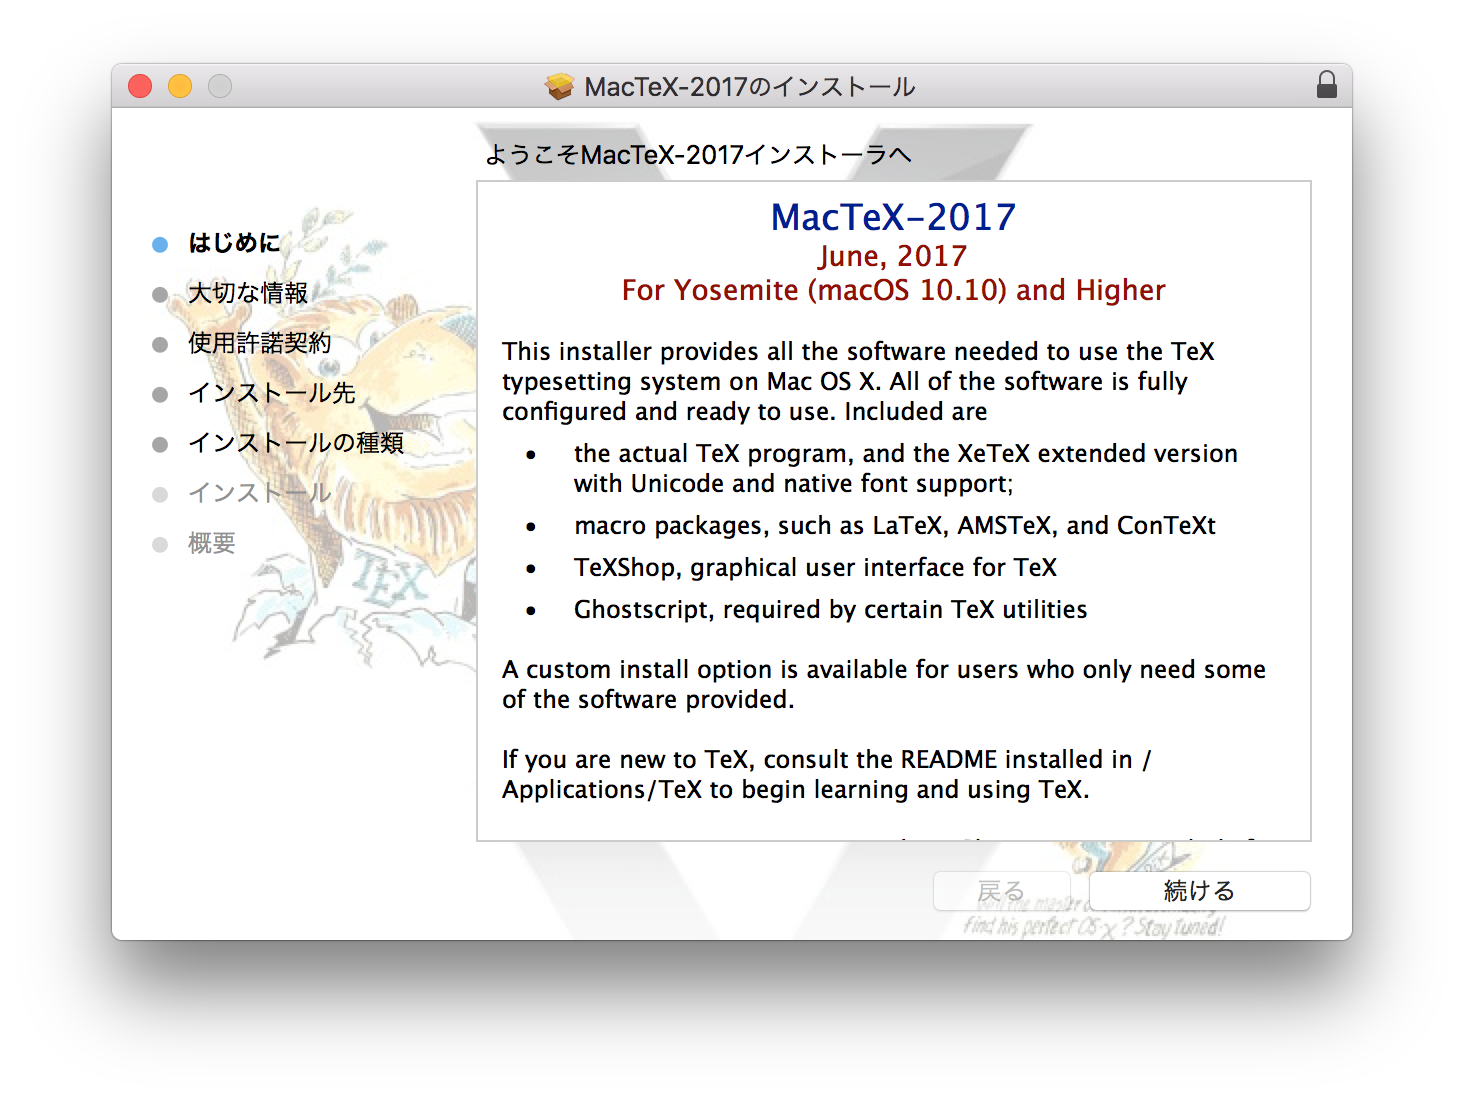
\includegraphics[width=10cm, ]{figs/image.png}
%   \end{center}
% \end{figure}

\chapter{移動ロボットの自己位置推定} \label{chapter:localization}

%%%%%%%%%%%%%%%%%%%%%%%%%%%%%%%%%%%%%%%%%%%%%%%%%%%%%%%%%%%%%%%%%%%%%%%%%%%%%%%%
本章では、ベイズフィルタによる移動ロボットの自己位置推定について定式化する。
また、ベイズフィルタの実装方法の1つであるMonte Carlo localization (以下MCL)について述べる。
本論文においても、移動ロボットの自己位置推定にはMCLが利用されるものとする。

% ベイズフィルタによる状態推定では、ロボットはセンサにより得た情報や自身の制御出力の履歴から、状態空間$\chi$内での現在の状態を確率的に推定する。
% ロボットの状態を表すパラメータについては様々存在するが、自己位置推定ではロボットの姿勢(位置と向き)を推定することを目的としている。
% 本論文では、二次元平面を低速で移動する対向二輪型のロボットを想定し、ロボットの二次元平面上における位置$x, y$と向き$\theta$をあわせた3次元の状態$(x, y, \theta)$の推定について扱う。


%%%%%%%%%%%%%%%%%%%%%%%%%%%%%%%%%%%%%%%%%%%%%%%%%%%%%%%%%%%%%%%%%%%%%%%%%%%%%%%%
\section{ベイズフィルタによる自己位置推定}

% ベイズフィルタによる自己位置推定では、式(\ref{bayes theorem})に示すベイズの定理を用いて、移動ロボットの位置を確率的に推定する。
% ベイズの定理は、事象$a, b$が起きる確率をそれぞれ$p(a), p(b)$としたときに、
% \begin{equation}
% \label{bayes theorem}
%   y = a
% \end{equation}



%%%%%%%%%%%%%%%%%%%%%%%%%%%%%%%%%%%%%%%%%%%%%%%%%%%%%%%%%%%%%%%%%%%%%%%%%%%%%%%%
\section{Monte Carlo localization (MCL)}

Monte Carlo localization (MCL)は、ベイズフィルタを理論的背景としたロボットの自己位置推定手法の1つである。
MCLでは、表現したい任意の空間上$\mathcal{X}$上に存在する確率密度関数を、空間上に散布した標本により表現することで、ロボットの姿勢を確率的に推定する。
この標本はパーティクル(粒子)と呼ばれ、ロボットの信念分布を表す確率密度関数$b_t(\bm{x})$を近似するように配置される。
各パーティクルは変数としてロボットと同次元の姿勢$\bm{x}$と重み$w$の情報を持っており、$N$個のパーティクルの集合は
\begin{equation}
\label{particles}
  % \Xi_{t} = \{ \xi^{(i)}_{t} = (\bm{x}^{(i)}_{t}, w^{(i)}_{t}) |i = 1,2,\dots,N \}
  \Xi = \{ \xi^{(i)} = (\bm{x}^{(i)}, w^{(i)}) |i = 1,2,\dots,N \}
\end{equation}
のように定義される。
基本的に全パーティクルの重みの合計は、常に
\begin{equation}
\label{weight_sum}
  \sum_{i=1}^{N}w^{(i)}_{t}=1
\end{equation}
を保つように実装される。

ロボットの状態を表す変数については様々存在するが、自己位置推定ではロボットの姿勢(位置と向き)を推定する。
本論文では、二次元平面を低速で移動する対向二輪型の移動ロボットを想定し、ロボットの二次元平面上における位置$(x, y)$と向き$\theta$をあわせた3次元の状態$\bm{x} = (x, y, \theta)$の推定について扱う。
したがって、ロボットの姿勢と同様に、パーティクルの姿勢はそれぞれ$\bm{x}^{(i)} = (x^{(i)}, y^{(i)}, \theta^{(i)})$となる。

% MCLには大きな利点が2つある。
% 1つ目の利点は、\ref{section:backglound}でも述べたとおり、多様な確率分布を表現できることである。
% もう1つの利点は、アルゴリズムが簡単なことである。
% したがって、比較的容易に実装することが可能である。

MCLのアルゴリズムは、主に次の4ステップからなる。
2から4を繰り返し行うことで逐次ロボットの姿勢を推定する。
\begin{enumerate}
  \item 初期化
  \item 動作による更新
  \item 計測による更新
  \item リサンプリング
\end{enumerate}

% ロボットの真の姿勢を$\bm{m}^{*}$とすると、ある時刻$t$におけるロボットの信念分布は$bel_{t}$と表現され、
% 本章のはじめで述べたとおり、本論文では移動ロボットの姿勢$\bm{x} = (x, y, \theta)$を推定することを想定したMCLを述べる。
% 各パーティクルはある時刻$t$におけるロボットの状態の具体的な事例であり、真の状態に対する1つの仮説と考えることができる。

% 標本はパーティクルと呼ばれる
% パーティクルはロボットの信念分布を近似するようにばらまかれる
% パーティクルは式で表現される
% 真の姿勢が存在する確率をしめす。
% これをパーティクルで表現すると


%%%%%%%%%%%%%%%%%%%%%%%%%%%%%%%%%%%%%%%%
\subsection{初期化}

初期化のステップでは、パーティクルの初期化を行う。
N個のパーティクルの初期姿勢$\bm{x}^{(i)}$を決定し、重み$w^{(i)}$を$1/N$とする。
パーティクルのばらまき方は、ロボットの初期の信念分布に従うように行う。
一般的には、以下のようなパーティクル初期姿勢の決定方法が用いられる。

ロボットを人間が自由に配置する場合など、初期姿勢が予め分かっている場合は、ロボットの信念分布をロボットが存在すると考えられる位置を平均とした正規分布と考え、
パーティクルの初期姿勢$\bm{x}^{(i)}$を平均$\mu$、分散$\Sigma$の正規分布に従うように決定する。
本論文における移動ロボットの自己位置推定では、状態$\bm{x}^{(i)}$が位置と向きからなる3次元のため、$\bm{\mu}$と$\Sigma$はそれぞれ3次元ベクトル、$3\times3$の分散共分散行列として扱う。
多くの場合$\bm{\mu}$と$\Sigma$はヒューリスティックに決定する。

一方、ロボットの初期位置が完全に不明なとき、ロボットの初期信念分布は状態空間$\mathcal{X}$全体の一様分布と考えられる。
その場合は、パーティクルの姿勢は一様分布に従うように配置する。

% MCLは、ロボットの制御出力や移動量、センサに含まれるノイズに頑健な推定が行える。
% しかし、想定を上回るノイズが混入した場合に、ロボットの真の姿勢$\bm{x}^{(*)}$とパーティクルの分布$\Xi$が大きく乖離することがある。
% MCLでは、パーティクルの分布がロボットの真の位置$\bm{x}^{*}$がから大きく離れることがある。
% このようなロボットの真の姿勢の周辺にパーティクルが存在しない状態は、「誘拐状態」と呼ばれる。
% 誘拐状態となったとき、一般的にはふたたびパーティクルが真の姿勢周辺に戻ることは少ないとされ、推定が大きく誤った状態が続く。
% そこで、融解状態から回復するための研究が複数行われている。
% 本論文では、ロボット


%%%%%%%%%%%%%%%%%%%%%%%%%%%%%%%%%%%%%%%%
\subsection{動作による更新}

動作による更新のステップでは、ベイズフィルタにおける予測ステップを、各パーティクルに対して行う。
移動ロボットの状態遷移にはノイズが伴うため、同様の制御入力でも試行ごとに異なる状態遷移結果となる。
したがって、ロボットが動作すると信念分布が広がることになる。
この広がった信念分布を表現するように、パーティクルの分布を更新する。
各パーティクルの状態をロボットの動作モデル
ロボットの状態遷移確率$p(\bm{x} | \bm{x}_{t-1}, \bm{u}_{t})$とすると、
動作後の各パーティクルの姿勢は
\begin{equation}
\label{particle trans prob}
  \bm{x}^{(i)}_{t} \sim p(\bm{x} | \bm{x}_{t-1}, \bm{u}_{t})
\end{equation}
のように更新される。


%%%%%%%%%%%%%%%%%%%%%%%%%%%%%%%%%%%%%%%%
\subsection{計測による更新}

計測による更新のステップでは、ベイズフィルタにおける計測更新ステップを行う。
センサにより得られた情報が、各パーティクルの状態で得られる確率を計算し、重み$w^{(i)}$を更新する。
重みの更新はベイズの定理を用いて
\begin{equation}
\label{weight}
  w^{(i)}_{t} = q(\bm{z}_{t} | \bm{x}^{(i)}_{t}) \hat{w}^{(i)}_{t}
\end{equation}
のように計算される。
尤度関数$q(z_{t} | \bm{x}^{(i)}_{t})$は、使用するセンサの観測モデルをもとに決定する。

現在、移動ロボットの自己位置推定のために、LiDARと呼ばれる光センサによる測距センサや、RGB-Dカメラが広く利用されている。
これらのセンサを自己位置推定位に用いるロボットは、条件が揃えば非常に正確な推定を行うことが可能である。
しかし、本論文では移動ロボットの状態推定が不確かなときに有効となるような行動決定の手法を提案することを目的としている。
したがって、移動ロボットが曖昧にしか状態推定を行えない状況を想定するために、ロボットはこれらのセンサを搭載していないものとする。

代わりに、ロボットはタスクの終了を検知することができるものとする。
この仮定は、\ref{chapter:method}章で述べる提案手法、およびその先行研究となるPFC法で必要となる。
ロボットは、自身がゴールに到達したか否かを各ステップごとに知ることができ、その情報を計測による更新に用いることができるものとする。

%%%%%%%%%%%%%%%%%%%%%%%%%%%%%%%%%%%%%%%%
\subsection{リサンプリング}
リサンプリングステップでは、パーティクルを再配置し重みを均一にする。
再配置するパーティクルは、重みに従った確率で選択される。
重みの小さいパーティクルを間引き、重みの大きいパーティクルの位置に多くのパーティクルを配置する。
この操作により、一箇所に重みが偏り続け推定の精度が下がることを防ぐ。

パーティクルの選択(サンプリング)にはいくつかの手法が存在する。
本論文では、系統抽出法によるリサンプリングを用いる。

\chapter{不確かさを考慮した行動決定} \label{chapter:pomdp}

本章では、不確かさを考慮した行動決定について述べる。
\ref{section:ロボットの行動決定}節では、ロボットの行動決定について述べる。
\ref{section:mdp}節では、状態が既知のロボットの行動決定を扱う枠組みである「マルコフ決定過程について述べる。
\ref{section:pomdp}節では、ロボットの状態が不確かにしか分からない状況での行動について扱う枠組みである
「部分観測マルコフ決定過程」について述べる。
\ref{section:q-mdp}節と\ref{section:PFC法}節では、
本研究の先行研究となる、$Q_{\rm MDP}$ value methodおよびPFC法について述べる。

% 本章では、不確かさを考慮した行動決定について述べる。
% まず、状態が既知のロボットの最適な行動決定を扱う枠組みである「マルコフ決定過程」について述べる。
% その後、ロボットの状態が不確かにしか分からない状況での最適な行動を扱う枠組みである「部分観測マルコフ決定過程」について述べる。
% 最後に、「部分観測マルコフ決定過程」を近似的に解く手法について、いくつかあるうち、本研究と関連のあるQ-MDP法およびPFC法について述べる。


%%%%%%%%%%%%%%%%%%%%%%%%%%%%%%%%%%%%%%%%%%%%%%%%%%%%%%%%%%%%%%%%%%%%%%%%%%%%%%%%
\section{ロボットの行動決定} \label{section:ロボットの行動決定}
本節では、ロボットの行動決定について考える。
本論文で扱うような移動ロボットの行動決定は、現在のロボットの位置から目的地までの最短経路を算出して移動する、「経路計画問題」として扱われる。
ダイクストラ法やA*法、人工ポテンシャル法といった多くの手法が提案されており、現在でも研究が行われている。
一般的にロボットの経路計画問題では、ロボットの観測や移動は決定論的なもとのして扱われ、経路が算出される。

しかし、これまで述べたとおり、移動ロボットは多くの不確かさを有している。
移動ロボットに最短の経路を算出して移動するだけでなく、これらの不確かさを考慮した上でさらに知的な動作を行わせる方法について考える必要がある。
たとえば、人間であれば、最短ではあるが危険でゴールに到達できる可能性が低い道よりも、多少遠回りではあるが高確率で安全にゴールできる道を選択するような、
「急がば回れ」が有効な場合も存在する。
あるいは、自身の位置が正しく把握できていない場合に、安全を優先し全く動かないでいるよりも、
多少の危険を冒しとりあえず行動してみてタスク達成を目指す方が有効であるような場合も考えられる。

このような知的な行動を、単純に経路計画問題として考えることは困難である。
そこで本章では、ロボットの移動と経路計画について、
より一般化した枠組みである(有限)マルコフ決定過程および部分観測マルコフ決定過程について述べる。

%%%%%%%%%%%%%%
%%%%ロボットの不確かさは大きく分けて、動作に関するものと観測に関するものの2つに分類できる。


%%%%%%%%%%%%%%%%%%%%%%%%%%%%%%%%%%%%%%%%%%%%%%%%%%%%%%%%%%%%%%%%%%%%%%%%%%%%%%%%
\section{マルコフ決定過程} \label{section:mdp}
本節では、移動ロボットの現在の自己位置$\bm{x} \in \mathcal{X}$が既知という前提での行動決定についての定式化を行う。
このような問題は、マルコフ決定過程(Markov decision process, MDP)という枠組みで議論される。
時間やロボットの状態等を連続系ではなく離散系で考える場合は、有限マルコフ決定過程と呼ばれる。

%%%%%%%%%%%%%%%%%%%%%%%%%%%%%%%%%%%%%%%%
\subsection{状態と終端状態}
\ref{chapter:localization}章で述べたものと同様に、
状態変数$x,y,\theta$からなる状態空間$\mathcal{X}$を定義する。
ロボットは自身の現在の状態ベクトル$\bm{x} \in \mathcal{X}$が分かっているものとし、観測の不確かさについては考慮しない。

ロボットのタスクには必ず終わりがあるとし、
ロボットの状態が、事前に定めたある状態になったときをタスクの終了とする。
このタスクが終了する状態は、終端状態と呼ばれ、終端状態の集合は$\mathcal{X}_f \subset \mathcal{X}$と表現される。
終端状態は、移動ロボットの経路計画問題における、ゴールや目標地点などのロボットが目指すべき望ましい状態だけでなく、陥りたくない状態も含まれる。

%%%%%%%%%%%%%%%%%%%%%%%%%%%%%%%%%%%%%%%%
\subsection{行動と状態遷移}
ロボットは有限子の制御指令の中から、一つを選択することで動作する。
MDPではこの制御指令のことを行動と呼ぶ。
ロボットの行動は$m$種類存在し、行動の集合は、
\begin{equation}
\label{action}
  \mathcal{A} = \{ a_{1}, a_{2}, \ldots , a_{m} \}
\end{equation}
と表現される。

時間は離散的に表現され、タスクの開始からは終わりまでは${0,1,2,\ldots,t_{f}} \equiv T$と定義される。
ロボットが最初に行動を選択する時刻を$t=0$とし、行動が実行されるたびに$t=1,2,\ldots$と次のステップへと進んでいく。
ロボットが終端状態に入りタスクが終了する時刻を$t_{f}$とする。
$t_{f}$は固定ではなく、タスク達成までにかかった時間により異なる。
また、「時刻$t-1$の状態」、「時刻$t$に遷移するために選択された行動」、「時刻$t$の状態」をそれぞれ$\bm{x}_{t-1}, a_{t}, \bm{x}_{t}$と表現する。
しかし、MDPで扱うシステムは時不変であるため、多くの場合$t$の具体的な値は重要でははない。
したがて、今後はこれらをそれぞれ$\bm{x}, a, \bm{x}^{\prime}$と表記する。

ロボットの状態$\bm{x}$は、ある行動$a$により状態$\bm{x}^{\prime}$へと遷移する。
状態の遷移にはノイズが含まれているものとし、状態と行動が同一の$(\bm{x}, a)$であっても、事後状態$\bm{x}^{\prime}$は各試行ごとに異なる。
ロボットの状態遷移は、マルコフ性を持ち、
\begin{equation}
\label{trans prob}
  \bm{x} \sim p(\bm{x} | \bm{x}_{t-1}, \bm{u}_t) (t=1,2,\ldots,t_{f})
\end{equation}
に従うものとする。
また、ロボットが$\bm{x}$から行動$a$により$\bm{x}^{\prime}$に遷移する確率を$p^{a}_{\bm{x}\bm{x}^{\prime}}$と表現する。
この確率$p^{a}_{\bm{x}\bm{x}^{\prime}}$が、$\bm{x}, a, \bm{x}^{\prime}$のあらゆる組に対して既知であり、時不変であると仮定する。

%%%%%%%%%%%%%%%%%%%%%%%%%%%%%%%%%%%%%%%%
\subsection{報酬} \label{subsection:reward}
状態$\bm{x}$で行動$a$を行った場合に、状態が$\bm{x}^{\prime}$に遷移した際に、その状態遷移に対して報酬を与える。
たとえば、移動ロボットではこの報酬は、行動一回ごとに消費する電力や時間などを設定する。
この報酬は、一つの実数値とし、$r^{a}_{\bm{x}\bm{x}^{\prime}} \in \mathbb{R}$と表現される。
評価の基準が多次元的の場合も、一つの実数となるように一元化し評価を行う。

%%%%%%%%%%%%%%%%%%%%%%%%%%%%%%%%%%%%%%%%
\subsection{評価}
ロボットがある状態$\bm{x}$からある終端状態$\bm{x}_{f} \in \mathcal{X}_{f}$に到達するまでの一連の状態遷移に対して評価を与える。
評価は、
\begin{equation}
\label{evaluation}
  J( \bm{x}_{0:t_{f}}, a_{1:t_{f}} ) = \sum^{t_{f}}_{t=1} r^{a}_{\bm{x}\bm{x}^{\prime}} + V(\bm{x}_{t_{f}})
\end{equation}
で定義される評価値の大きさで行う。
$r^{a}_{\bm{x}\bm{x}^{\prime}}$は、\ref{subsection:reward}項で述べた報酬である。
$V(\bm{x}_{t_{f}})$は終端状態の価値とし、事前に目的に応じて与えられるものとする。
ロボットが目指すゴールや目標地点とする場合、$0$を設定する。
逆に、ロボットがその状態になった場合タスクが失敗として終了するような、絶対に陥ってほしくない状態として設定する場合、非常に小さい値を設定する。

本論文では、この評価値$J$を最大化する一連の状態遷移を、最適な制御とする。
状態遷移にはノイズが伴うため、同じ姿勢$\bm{x}_{0}$から常に最適となるような行動をとったとしても、試行ごとに評価値$J$は異なる。
そのため、ある状態から終端状態までの一連の状態遷移に対する評価$J$は、期待値として考える。

%%%%%%%%%%%%%%%%%%%%%%%%%%%%%%%%%%%%%%%%
\subsection{最適方策}
ある状態における、Jの期待値を最大化するための行動を与える関数
\begin{equation}
\label{policy}
  \Pi : \mathcal{X} \rightarrow \mathcal{A}
\end{equation}
を定義する。
この関数$\Pi$は最適方策と呼ばれる。
最適方策$\Pi$が決まると、任意の状態$\bm{x}$でロボットが取るべき行動は、
\begin{equation}
\label{oprimal action}
  a = \Pi(\bm{x}) \;\;\;\; (\forall \bm{x} \in \mathcal{X})
\end{equation}
と自動的に決まる。

%%%%%%%%%%%%%%%%%%%%%%%%%%%%%%%%%%%%%%%%
\subsection{最適価値関数}
また、ある状態に対して評価値の期待値$J$を与える関数
\begin{equation}
\label{value function}
  V : \mathcal{X} \rightarrow \mathbb{R}
\end{equation}
は、最適価値関数と呼ばれる。
$V(\bm{x})$は、$\bm{x}$が初期の状態でも、タスクにおける途中の状態でも変わらない。
終端状態の価値$V(\bm{x}_{t_{f}})$は、この最適価値関数に含まれる。


%%%%%%%%%%%%%%%%%%%%%%%%%%%%%%%%%%%%%%%%%%%%%%%%%%%%%%%%%%%%%%%%%%%%%%%%%%%%%%%%
\section{部分観測マルコフ決定過程} \label{section:pomdp}
本節では、移動ロボットの現在の状態が不確かな中での行動決定について述べる。
このような問題は、部分観測マルコフ決定過程(partially observable Markov decision process, POMDP)という枠組みで研究が行われている。

POMDPがMDPと異なる点は、ロボットが真の状態が分かっていないという点にある。
ロボットはMDP同様、評価値$J$を最小化するように終端状態にたどり着くことを目的とする。
しかし、ロボットの姿勢$\bm{x}$が未知であるため、最適方策$\Pi(\bm{x})$を使用することができない。
したがって、$\bm{x}$の代わりにその場で得られる情報をもとに行動を決定する必要がある。
ロボットがこれまで行ってきた行動の履歴$a_{1:t}$、それまでに得た観測の情報$z_{1:t}$、およびそれまでに得た報酬の履歴$r_{1:t}$から決定される方策は
\begin{equation}
\label{policy pomdp}
  a_{t+1} = \Pi_{\rm POMDP} (a_{1:t}, \bm{z}_{1:t}, r_{1:t})
\end{equation}
と定義される。

ロボットが行動を決定するとき、その時点での状態推定の不確かさを考慮したい場合、関数
\begin{equation}
\label{policy belief}
  a_{t+1} = \Pi_{\rm b} (b_{t})
\end{equation}
を考えればよいことになる。
この関数は、ロボットの姿勢を状態とするのではなく、ロボットの信念分布自体をひとつの状態としてみなし、
とるべき行動をロボットの現在の信念分布から決定する。
状態としてみなされる信念分布は、信念状態と呼ばれる。

このように信念の分布をひとつの状態とみなすことで、POMDPの問題をMDPの問題として考えることができる。
信念状態を用いることでPOMDPをMDPとして考える方法は、belief MDPと呼ばれる\cite{kaelbling1998}。
しかし、信念状態の数は非常に膨大であり、最適方策を得ることは通常不可能とされている。
そこで、最適ではなくとも、全く不確かさを考慮しないときよりは優れた行動を近似的に得る、という手法を考えることが有効となる。


%%%%%%%%%%%%%%%%%%%%%%%%%%%%%%%%%%%%%%%%%%%%%%%%%%%%%%%%%%%%%%%%%%%%%%%%%%%%%%%%
\section{Q-MDP} \label{section:q-mdp}
本節では、Q-MDPについて述べる。
この手法は、Littmanらにより\cite{littman1995}で提案され、Uedaらによって\cite{}でロボットに適用された。

Q-MDP法は、観測の不確かさを考慮せずに、MDP問題として解かれた最適価値関数と、信念分布から行動を決定する。
各行動に対する期待値計算を行い、最も期待値が高くなるような行動を選択する。
信念分布がパーティクルにより近似されているとき、期待値は、
\begin{equation}
\label{equation:q-mdp}
  Q_{\rm PFC}(a, b) = \sum_{i=1}^{N} w^{(i)}
                      \left[r^{a}_{s^{(i)} s^{\prime}} + V(s^{\prime}) \right]
\end{equation}
のように計算される。
この期待値を全行動$a \in \mathcal{A}$に対して計算し、最大となる行動を
\begin{equation}
\label{equation:pi q-mdp}
  \Pi_{Q_{\rm MDP}}(b) = \argmax_{a \in \mathcal{A}} Q_{\rm MDP}(a, b)
\end{equation}
のように決定する。

Q-MDP法は、UedaらによってRoboCupの四足歩行リーグのゴールキーパーのロボットへと適用され、有効性が示されている\cite{ueda2003iros}。
しかし、本論文で扱うような移動ロボットでは、ローカルミニマムによる行動の停滞が頻繁に起こるQ-MDP法は、あまり有効な方法とは言えない。
また、\ref{section:related works}節で述べた沿岸航法の探索動作のような、

%%%%%%%%%%%%%%%%%%%%%%%%%%%%%%%%%%%%%%%%%%%%%%%%%%%%%%%%%%%%%%%%%%%%%%%%%%%%%%%%
\section{Probabilistic Flow Control} \label{section:PFC法}
本節では、PFC(Probabilistic Flow Control)法について述べる。
この手法は、Uedaにより\cite{ueda2015}で提案されている。

PFC法では、行動評価の式を
\begin{equation}
\label{equation:pfc}
  Q_{\rm PFC}(a, b) = \sum_{i=1}^{N} \frac{ w^{(i)} }{ V(\V{x}^{(i)})^{m} }
                      \left[r^{a}_{\V{x}^{(i)} \V{x}^{\prime}} + V(\V{x}^{\prime}) \right]
\end{equation}
のように変更することで、ゴールに近いパーティクルが行動決定に与える影響を大きくし、ロボットのゴール探索動作を生成した。
ここで、$m$は\cite{ueda2018searching}で導入されたパラメータで、ゴールに近いパーティクルの行動決定への影響度を決定する。
ロボットはパーティクル分布を徐々にゴールへと流し込むように動作し、分布の中にロボットが存在する場合、ロボットの流れに従いゴールへと到達する。
この手法は、知的な探索動作を生成し、かつQ-MDP法で問題となっていたローカルミニマムによる行動停滞の頻度の低下も確認されており、
移動ロボットのナビゲーションタスクに対し有効である。


%%% 参考文献 %%%
% よほどのことが無い限りet al.は使わないことにしましょう
\bibliographystyle{jualpha}
\bibliography{./references}

\newpage
\printindex

\end{document}
